\chapter{Design and Methodology}
\label{cha:design-and-method}

Based on our analysis and the information we want to collect, we decided on the following architecture for our system [\ref{fig:architecture1}]:

\begin{figure}[h!]
	\centering
	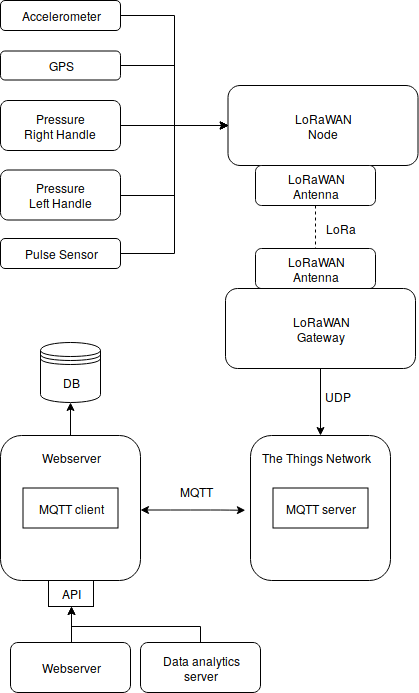
\includegraphics[width=0.9\linewidth]{gfx/architecture_design_and_methology_h}
	\caption{Proposed architecture}
	\label{fig:architecture1}
\end{figure}

\section{Components and their interactions}


	\subsection{LoRaWAN node}
		Polls the sensors in predefined intervals and sends them through LoRaWAN every few minutes

	\subsection{LoRaWAN gateway}
		Receives LoRaWAN packets and relays them to "The Things Network" through the Semtech UDP protocol

	\subsection{The Things Network (TTN)}\label{ttn_description}
		It is possible to have our gateway communicate directly with our server, but we decided to use TTN because it provides some very useful features out of the box, some of them being:

		\begin{itemize}
			\item Node authentication
			\item Packet deserialization
			\item Integration with MQTT, HTTP, Google Cloud, Amazon AWS and Azure
			\item Encryption
			\item Has thousands of registered gateways
		\end{itemize}

		TTN has become the standard in LoRaWAN applications, due to its unparalleled potencial for scalability, integration and security. In our case it deserializes the packets coming from the gateways and publishes them in an MQTT broker 

	\subsection{Server}
		The server will subscribe to the MQTT broker on TTN and store the information received from there, while also exposing an API that can be used, for example, to have other services process the data and display it to the interested parties
	
	\newpage
	This interaction of the mentioned components is visualized in the following [\ref{fig:sequenceDiagram}]: 
	\begin{figure}[h!]
		\centering
		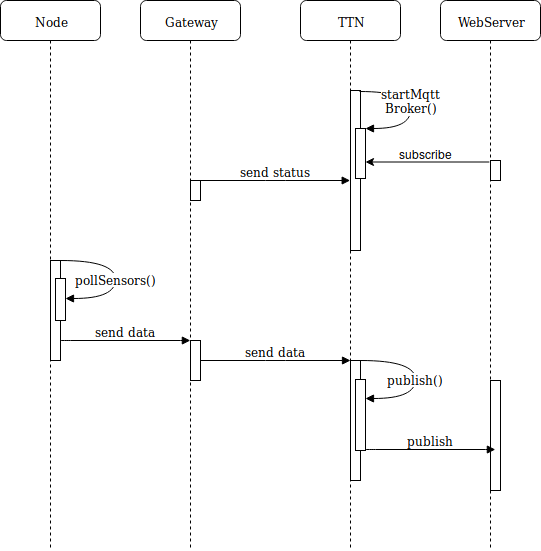
\includegraphics[width=0.9\linewidth]{gfx/sequenceDiagram.png}
		\caption{Proposed architecture}
		\label{fig:sequenceDiagram}
	\end{figure}
	
	
\section{Experiments}
	In order to test the previously mentioned quality parameters and thus our hypothesis, we designed the following experiments:

	\subsection{Normal Usage}
		In order to test the consistency and accuracy of our readings, the reliability of the whole system, its latency, and its energy consumption when in use, we have to use the walker and analyse what output we get. We will thus do two runs of 30 minutes, doing as much as possible to keep all the factors constant and save all the information we get. We can then use the sensor readings to find out our consistency and accuracy, the percentage of packets dropped for latency, the delay between them for latency and the energy used for energy consumption.

	\subsection{Idle Energy Consumption}
		We will leave the walker idle for around 12 hours while measuring its energy comsumption.
		We can then calculate how much energy the node consumes per hour both idle and in use (above experiment) and conclude how much it will last on common 9V batteries.

	\subsection{Integrating the GPS sensor}
		In order to test the modularity of the system, we will deliberately only integrate the GPS sensor in the testing phase of the project, this way we can measure how much time it takes and analyse the complications brought by doing so.

	\subsection{Testing the GPS sensor}
		It would be hard for us to integrate the GPS data testing with the bigger experiment mentioned above, due to the fact that we would have to be outside for it to work and the sensors we are using break very easily, so we are divising an experiment just for it.
		We are going to get the location of the walker 40 times and do some statistical analysis on that data.

	\subsection{Setting up the Arduino from scratch}
		Due to the fact that we only have one LoRaWAN hat for the Arduino, we are not able to have two setups running simultaneously, so we will re-register the Arduino in "The Things Network" and re-upload the code to it, measuring how much time the process takes. We will do it once without practicing the process, and then one more time when we know exacly which steps to take. This experiment is the closest we can get to testing the scalability of our system.

	\subsection{Disconnecting cables}
		In order to test serviceability, we will have someone disconnect random cables connecting the sensors to the node and we will then have another member of the team get the system back up and running while we measure the time it takes.

	\subsection{Finding maximimum throughput}
		We will increase the ammount of bytes being sent by the node until they no longer arrive, this will allow us to discover the maximum amount of information we are able to send in each packet.

%%% Local Variables:
%%% mode: latex
%%% TeX-master: "../ClassicThesis"
%%% End:
